\documentclass[9pt,twocolumn,twoside]{pnas-new}
% Use the lineno option to display guide line numbers if required.
% Note that the use of elements such as single-column equations
% may affect the guide line number alignment. 

\templatetype{pnasresearcharticle} % Choose template 
% {pnasresearcharticle} = Template for a two-column research article
% {pnasmathematics} = Template for a one-column mathematics article
% {pnasinvited} = Template for a PNAS invited submission

\title{Adaptation lies at the nexus of consistency and optimality in olfactory sensing of sparse signals}

% Use letters for affiliations, numbers to show equal authorship (if applicable) and to indicate the corresponding author
\author[a,c,1]{Author One}
\author[b,1,2]{Author Two} 
\author[a]{Author Three}

\affil[a]{Affiliation One}
\affil[b]{Affiliation Two}
\affil[c]{Affiliation Three}

% Please give the surname of the lead author for the running footer
\leadauthor{Lead author last name} 

% Please add here a significance statement to explain the relevance of your work
\significancestatement{Authors must submit a 120-word maximum statement about the significance of their research paper written at a level understandable to an undergraduate educated scientist outside their field of speciality. The primary goal of the Significance Statement is to explain the relevance of the work in broad context to a broad readership. The Significance Statement appears in the paper itself and is required for all research papers.}

% Please include corresponding author, author contribution and author declaration information
\authorcontributions{Please provide details of author contributions here.}
\authordeclaration{Please declare any conflict of interest here.}
\equalauthors{\textsuperscript{1}A.O.(Author One) and A.T. (Author Two) contributed equally to this work (remove if not applicable).}
\correspondingauthor{\textsuperscript{2}To whom correspondence should be addressed. E-mail: author.two\@email.com}

% Keywords are not mandatory, but authors are strongly encouraged to provide them. If provided, please include two to five keywords, separated by the pipe symbol, e.g:
\keywords{Keyword 1 $|$ Keyword 2 $|$ Keyword 3 $|$ ...} 

\begin{abstract}
Please provide an abstract of no more than 250 words in a single paragraph. Abstracts should explain to the general reader the major contributions of the article. References in the abstract must be cited in full within the abstract itself and cited in the text.
\end{abstract}

\dates{This manuscript was compiled on \today}
\doi{\url{www.pnas.org/cgi/doi/10.1073/pnas.XXXXXXXXXX}}


%% Manual commands
\relpenalty=9999
\binoppenalty=9999

\begin{document}

% Optional adjustment to line up main text (after abstract) of first page with line numbers, when using both lineno and twocolumn options.
% You should only change this length when you've finalised the article contents.
\verticaladjustment{-2pt}

\maketitle
\thispagestyle{firststyle}
\ifthenelse{\boolean{shortarticle}}{\ifthenelse{\boolean{singlecolumn}}{\abscontentformatted}{\abscontent}}{}

% If your first paragraph (i.e. with the \dropcap) contains a list environment (quote, quotation, theorem, definition, enumerate, itemize...), the line after the list may have some extra indentation. If this is the case, add \parshape=0 to the end of the list environment.
%Note: please start your introduction without including the word ``Introduction'' as a section heading (except for math articles in the Physical Sciences section); this heading is implied in the first paragraphs. 

\dropcap{I}ntroduction. 

%%%%%%%%%%%%%%%%%%%%%%%%%%%%%%%%%%%%%%%%%%%%%%%%%%%%%%%%%%%%%%%%%%%%%%
%%%%%%%%%%%%%%%%%				MODEL			%%%%%%%%%%%%%%%%%%%%%%
%%%%%%%%%%%%%%%%%%%%%%%%%%%%%%%%%%%%%%%%%%%%%%%%%%%%%%%%%%%%%%%%%%%%%%


\section*{Model}

\subsection*{Discrete-state stochastic olfactory receptor model}

We describe the sensory system by a stochastic discrete-state model, analogous to those used in describing ligand binding to chemoreceptor homodimers in bacterial chemotaxis. Deferring for now the effect of temporal fluctuations, we treat the dynamics in steady state, where the combination of odorant (un)binding and receptor (in)activation conspire to produce mean-field activity levels in response to given odorant stimuli. Here, we model the sensory complex as a single unit consisting of an olfactory receptor (OR) and and a co-receptor protein Orco, known to be expressed in the majority of insect ORNs, including all OR-expressing ORNs in \textit{drosophila}. This Or-Orco complex may exist in either an activated or inactivated state, and may be independently bound or unbound to volatile odorant molecular signals $s_i$. Binding obeys a stochastic jump process, where the affinity for binding is higher when activated. To simplify the analysis, we assume that a given receptor complex $R^\rho$ may bind at most a single monomolecular odorant at one time. Among a selection of $N$ such odorants, $R^{\rho}$ may therefore live in one of $N+1$ inactivated states with associated concentrations, $\{[R^\rho], [R^\rho s_1], [R^\rho s_2],...,[R^\rho  s_N]\}$ or $N+1$ activated states with concentrations $\{[R^\rho _*], [R^\rho _*s_1], [R^\rho _*s_2],...,[R^\rho _*s_N]\}$. 
Assuming that the binding of odors is faster than the time to activate or deactivate, the former is approximately quasistatic, with steady state probabilities
\begin{align}
p_{\text b}^{\rho i} = \frac{\frac{[s_i]}{K^{\rho i}}}{1 + \sum_i^N \frac{[s_i]}{K^{\rho i}}}, \qquad  
p_{\text b*}^{\rho i} = \frac{\frac{[s_i]}{K_*^{\rho i}}}{1 + \sum_i^N \frac{[s_i]}{K_*^{\rho i}}},
\label{eq:steady_state_binding_probabilities}
\end{align}
when (in)activated, and where $K^{\rho i}$ and $K^{\rho i}_*$ are the corresponding disassociation constants of the individual jump processes. Likewise, the activation kinetics when (un)bound obey Master equations
\begin{align}
\frac{d[R_*^\rho]}{dt} &= w_{\text u +}^\rho [R^\rho] - w_{\text u -}^\rho [R_*^\rho] \\
\frac{d[R_*^\rho s_i]}{dt} &= w_{\text b +}^{\rho i} [R^\rho s_i] - w_{\text b -}^{\rho i} [R_*^\rho s_i]
\label{eq:activation_master_equations}
\end{align}

When unbound, the free energy difference between inactivated and activated receptors is signal-independent, but may be distinct for differing receptors; we denote these as $\epsilon^\rho_{\text u}\equiv\ln(w^\rho_{\text u +}/w^\rho_{\text u -})$. Detailed balance enforced on 4-cycles involving a single ligand, therefore, demands 
$K_*^{\rho i}w_{\text b+}^\rho w_{\text u -}^\rho / 
K^{\rho i} w_{\text u +}^\rho w_{\text b -}^\rho \equiv 1$, 
whereby the free energy difference between activated and inactivated states when bound depends on the disassociation constants:
$\ln(w^{\rho i}_{\text b +}/w^{\rho i}_{\text b -}) \equiv
\epsilon_{\text b}^{\rho i} =
\epsilon_{\text u}^{\rho i} + \log(K_*^{\rho i}/K^{\rho i})$. 

In the mean-field limit, the collective action of binding and activation produces an activity level for each receptor: a sum of the concentrations of all activated states, bound or unbound. 
%$a^\rho = [R^\rho_*] + \sum_i^N[R^\rho_* s_i]$, 
The dynamics of these activity levels then obeys a linear rate equation, which in steady state relaxes to
\begin{align}
\bar a^\rho(\{[s_i]\}, \epsilon_{\text {u}}^\rho) = \left( 1 + e^{\epsilon^\rho_{\text u}}\frac{1 + \sum_{i=1}^N [s_i]/K^{\rho i}}{1 + \sum_{i=1}^N [s_i]/K_*^{\rho i}}\right)^{-1}.
\label{eq:steady_state_activity}
\end{align}
This expression is a simple generalization of the analogous expression for a 4-state receptor model with a single binding site. 
%In the limit that the system has a higher affinity for activation when bound than when unbound, we have $KK^{\rho i}_* \ll KK^{\rho i}$, and Eq.~\ref{eq:steady_state_activity} reduces to $\bar a^\rho = (1 + e^{\epsilon_{\text b}^\rho})

At a much larger timescale than odorant binding and receptor complex activation, the free energies $\epsilon^\rho_{\text u}$ may be modulated by adaptive feedback, adjusting in such a way to, ideally, maintain the sensitivity and range of the ORNs in response to fluctuating environments. We model this in a minimal fashion via $\dot \epsilon_{\text u}^\rho = \beta^\rho(a_0^\rho - \bar a^\rho)$, which assumes that the activity levels may decay at differing rates and to differing backgrounds for distinct receptor complexes $R^\rho$. {\color {blue} Say something about WL here?}


%$\dot a^\rho = (1 - a^\rho)w_+^\rho + w_-^\rho a$, where the transition rates $w^\rho_+$ and $w_-^\rho$ are appropriately weighted sums of $w_{\text u +}$, $w_{\text u -}$, $w_{\text u}$, and $w_{}
%$w_+ = (1-\sum_i^N p^{\rho i}_{\text b})w_{\text u +}^\rho +  \sum_i^N p^{\rho i}_{\text b} w_{\text b +}^{\rho i}$ and $w_- = (1-\sum_i^N p^{\rho i}_{\text b})w_{\text u -}^\rho +  \sum_i^N p^{\rho i}_{\text b} w_{\text b -}^{\rho i}$.
%The associated master equations for $2N$ possible 2-state jump processes are
%\begin{align}
%\frac{d [R^\rho s_i]}{dt} &= k_-^{\rho i} s_i [R^\rho] - k_+^{\rho i} [R^\rho s_i] \\
%\frac{d [R^\rho_* s_i]}{dt} &= k_-^{\rho i} s_i [R_*^\rho] - k_+^{\rho i} [R_*^\rho s_i] 
%\end{align} 

\subsection*{Decoding sparse signals}
It has been observed that despite the vast array of distinct odors between which humans and other animals can discriminate, individual odors found in the natural environment contain only a handful of monomolecular components -- odor signals are \textit{sparse} in the $N$-dimensional space of constituent volatile molecules. Even without other mechanisms such as temporal dynamics, the theory of compressed sensing might explain how so many odors are reliably discriminated by a few dozen ORNs. In compressed sensing, signal sparsity acts as a regulator that renders the inverse problem well-posed; if the sensor output $\mathbf a$ were generated from signals $\mathbf s$ through a set of linear observations, $\mathbf s$ could be recovered with fidelity given fewer than $N$ measurements -- an otherwise underdetermined problem. %Specifically, if the activity is generated from the signal without the addition of noise, then the original signal $\mathbf s$ can be decoded by 
Specifically, this estimate is the vector which minimizes the $L_1$ norm of the signal subject to the measured activity:
\begin{align}
\hat {\mathbf s} = \arg \min \sum_i^N |s_i| \quad \text {s.t.  } \mathbf a = \mathbf M \mathbf s,
\label{eq:compressed_sensing_formulation}
\end{align}
where $\mathbf M$ is an $M$x$N$ measurement matrix.


\begin{figure}%[tbhp]
	\centering
	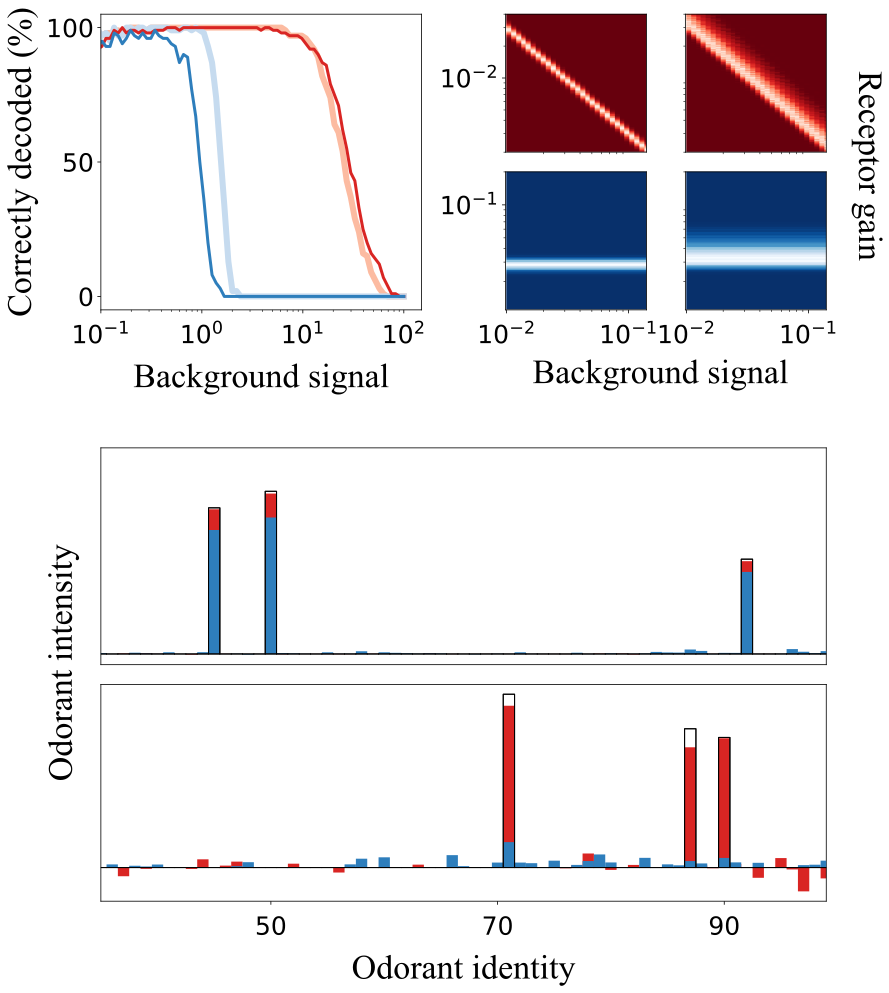
\includegraphics[width=.8\linewidth]{figures/signal_decoding_weber_law/signal_decoding_weber_law}
	\caption{test size.}
	\label{fig:frog}
\end{figure}

But odor binding and transduction are nonlinear processes: olfactory encoding cannot be described by the simple linear input-output relation $a^\rho = M^{\rho i} s_i$, rather a more general formulation such as the steady state expression Eq.~\ref{eq:steady_state_activity}. One could in principle carry out the optimization in Eq.~\ref{eq:compressed_sensing_formulation} with the replacement of the linear constraint,  but the recovery of $\mathbf s$ is not straightforward as nonlinear programming contains no guarantees on convexity, and may well converge to a local minimum. To incorporate the odor binding dynamics in a sensible way, we assume the activity levels relax to their steady state values, Eq.~\ref{eq:steady_state_activity}, but use only a first-order approximation of the full binding and activation process for decoding. 

Adopting the viewpoint that the neural system can learn the mean background stimulus, we linearize fluctuations of the sparse odor signals around a known background $\bar{\mathbf s}$, estimating only the fluctuations $\Delta \mathbf s = \mathbf s - \bar{\mathbf s}$ via Eq.~\ref{eq:compressed_sensing_formulation}. In the limit $K_*^{\rho i} \ll s_i \ll K^{\rho i}$, this gives a measurement matrix $M^{\rho i} = (e^{\epsilon^\rho_{\text u}}/K_*^{\rho i})/(\sum_{i=1}^N s_i^0/K_*^{\rho i} + e^{\epsilon^\rho_{\text u}})^2$. 

\section*{Results}

\subsection*{An arbitrary activity distribution naturally preserves Weber-Law scaling} 


Compressed sensing relies on both input vector sparsity and measurement matrix decoherence, the latter of which implies a degree of randomness in $\mathbf M$. Sensory receptor systems such as ORNs are known to adapt their gain levels to maximize sensitivity to quasi-static backgrounds, and it is suggestive that if ORNs are indeed decoding sparse odor signals, the linearized measurement matrix -- a joint function of free energies $\epsilon_{\text u}^\rho$, activated disassociation constants $K_*^{\rho i}$, and background signals $s_0$ -- is statistically distributed in such a way to optimally preserve sensitivity over a broad range of backgrounds. 

\begin{figure}%[tbhp]
	\centering
	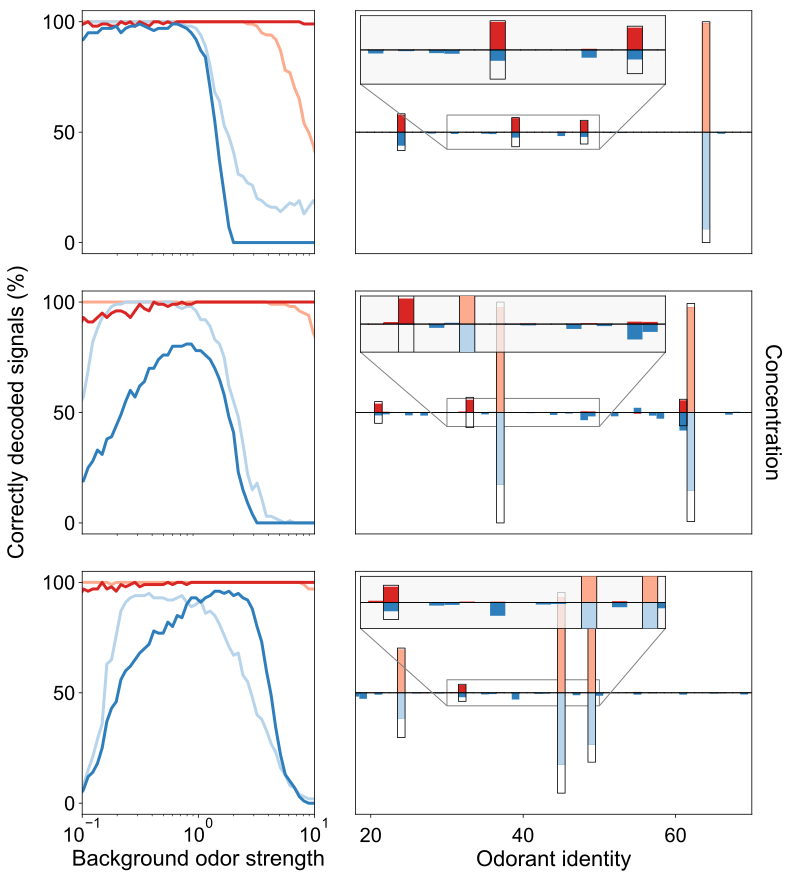
\includegraphics[width=.85\linewidth]{figures/signal_discrimination_weber_law/signal_discrimination_weber_law}
	\caption{test size.}
	\label{fig:frog}
\end{figure}

On the one hand, we might assign a particular prior on the disassociation matrices $K_*^{\rho i}$. Alternatively, we may adopt the viewpoint that in response to fluctuating backgrounds, the sensory system adapts $\epsilon^\rho_0$ dynamically to maintain the output levels $\bar a^\rho$ to a set range, and that this range is inherently tuned to sparsity. This viewpoint may be more in line with previous studies and subsequent re-analyses of drosophila ORNs indicating that firing rates appear to follow a single distribution across ORN types and mean signal magnitudes. 

Adopting this perspective, let us assume that the activity response of a given olfactory receptor $\rho$ to individual monomolecular odorants of a fixed concentration $s_0$ is approximately normally distributed (truncated outside of the closed interval [0, 1] in accordance with Eq.~\ref{eq:steady_state_activity}):
\begin{align}
\bar a^\rho([s_i] = s_0) \sim \mathcal N(\mu_\rho, \sigma_\rho)
\label{eq:monomolecular_activity_levels}
\end{align} 
The assumption of Gaussian-distributed activity levels, however, imply non-normal statistics for the disassociation matrices. In the limit of disparate binding affinities for the activated and inactivated receptors, $K^{\rho i}_* \ll s_i \ll K^{\rho i}$, the probability density function for $K^{\rho i}$ for a given receptor $\rho$ is
\begin{align}
p_\rho(K_*^{\rho i} = x)  \sim \frac{e^{-\left[\mu_\rho - \frac{(x/C_\rho + 1)^{-1}}{\sqrt{2\pi \sigma^2}}\right]^2}}{(x/C_\rho + 1)^2}, 
\label{eq:distribution_Kk2_normal_activity}
\end{align}
where $C_\rho = e^{-\epsilon_{\text u}^\rho}s_0$. 

As the mean odorant concentration is modulated, activity levels respond dynamically to fast fluctuations. Simultaneously, $\epsilon_{\text u}^\rho$ adjusts, slowly driving activity levels back to a latent firing rate, around 30 Hz for typical ORNs. The implication of Eq.~\ref{eq:distribution_Kk2_normal_activity} is $\bar a^\rho$ cannot be independent of background signal, unless $C_\rho$ is fixed. Yet the constancy of $C_\rho$ is just the adaptive scaling
\begin{align}
\epsilon_{\text u}^\rho \sim \log(s_0),
\end{align}
which is Weber's Law itself. The implication is that log-sensing adaptation arises naturally and consistently from normally-distributed receptor response to monomolecular signals. {\color {blue} Same for any distribution really; however the interplay of mean and variance cold be meaningful.}

To what extent is adaptive scaling necessary in maintaining coding fidelity? To probe this, 

\subsection*{The optimal ORN tuning curve}

Of equal importance, the connection between individual ORN activity levels and the decoding process via Eqs.~\ref{eq:steady_state_activity},~\ref{eq:compressed_sensing_formulation}, and~\ref{eq:distribution_Kk2_normal_activity} suggests that the precise shape of ORN tuning curves -- and the diversity of these curves across distinct receptors -- may in fact rely more fundamentally on maintaining activity levels in optimal regimes. To explore the effect of tuning curve shape and diversity on decoding fidelity, we first assume that all receptors exhibit identical, narrow tuning curves, $\mu_\rho \equiv \mu_{[\rho]}$ and $\sigma_\rho \equiv \sigma_{[\rho]}$, where $\sigma_{[\rho]}\sim 0.01$. We optimize the decoding error over $\mu_{[\rho]}$, using two separate metrics: the percentage of accurately estimated nonzero components, as well as the percentage of properly estimated zero components (see Materials and Methods). 


%In addition to providing a testable prediction, the distribution of disassociation constants, Eq.~\ref{eq:distribution_Kk2_normal_activity}, is quite general in that any given distribution of $a^\rho$ will produce an inverse distribution in $K^{\rho i}_*$. When applied to the exponential family, such inverse distributions are necessarily dominated by $\sim 1/x^2$ behavior away from their central mode; this long-tail behavior would could itself account for non-normal diversity in sensory mechanisms. 

\subsection*{Receptor diversity }

\subsection*{Insensitivity to background w/ Gaussian K?}





\subsection*{blh}

asd
\subsection*{Author Affiliations}

Include department, institution, and complete address, with the ZIP/postal code, for each author. Use lower case letters to match authors with institutions, as shown in the example. Authors with an ORCID ID may supply this information at submission.

\subsection*{Submitting Manuscripts}

All authors must submit their articles at \href{http://www.pnascentral.org/cgi-bin/main.plex}{PNAScentral}. If you are using Overleaf to write your article, you can use the ``Submit to PNAS'' option in the top bar of the editor window. 

\subsection*{Format}

Many authors find it useful to organize their manuscripts with the following order of sections;  Title, Author Affiliation, Keywords, Abstract, Significance Statement, Results, Discussion, Materials and methods, Acknowledgments, and References. Other orders and headings are permitted.

\subsection*{Manuscript Length}

PNAS generally uses a two-column format averaging 67 characters, including spaces, per line. The maximum length of a Direct Submission research article is six pages and a PNAS PLUS research article is ten pages including all text, spaces, and the number of characters displaced by figures, tables, and equations.  When submitting tables, figures, and/or equations in addition to text, keep the text for your manuscript under 39,000 characters (including spaces) for Direct Submissions and 72,000 characters (including spaces) for PNAS PLUS.

\subsection*{References}

References should be cited in numerical order as they appear in text; this will be done automatically via bibtex, e.g. \cite{belkin2002using} and \cite{berard1994embedding,coifman2005geometric}. All references, including for the SI, should be included in the main manuscript file. References appearing in both sections should not be duplicated.  SI references included in tables should be included with the main reference section. 

\subsection*{Data Archival}

PNAS must be able to archive the data essential to a published article. Where such archiving is not possible, deposition of data in public databases, such as GenBank, ArrayExpress, Protein Data Bank, Unidata, and others outlined in the Information for Authors, is acceptable.

\subsection*{Language-Editing Services}
Prior to submission, authors who believe their manuscripts would benefit from professional editing are encouraged to use a language-editing service (see list at www.pnas.org/site/authors/language-editing.xhtml). PNAS does not take responsibility for or endorse these services, and their use has no bearing on acceptance of a manuscript for publication. 

\begin{figure}%[tbhp]
\centering
\includegraphics[width=.8\linewidth]{figures/frog}
\caption{Placeholder image of a frog with a long example caption to show justification setting.}
\label{fig:frog}
\end{figure}


\begin{SCfigure*}[\sidecaptionrelwidth][t]
\centering
\includegraphics[width=11.4cm,height=11.4cm]{figures/frog}
\caption{This caption would be placed at the side of the figure, rather than below it.}\label{fig:side}
\end{SCfigure*}

\subsection*{Digital Figures}
\label{sec:figures}

Only TIFF, EPS, and high-resolution PDF for Mac or PC are allowed for figures that will appear in the main text, and images must be final size. Authors may submit U3D or PRC files for 3D images; these must be accompanied by 2D representations in TIFF, EPS, or high-resolution PDF format.  Color images must be in RGB (red, green, blue) mode. Include the font files for any text. 

Figures and Tables should be labelled and referenced in the standard way using the \verb|\label{}| and \verb|\ref{}| commands.

Figure \ref{fig:frog} shows an example of how to insert a column-wide figure. To insert a figure wider than one column, please use the \verb|\begin{figure*}...\end{figure*}| environment. Figures wider than one column should be sized to 11.4 cm or 17.8 cm wide. Use \verb|\begin{SCfigure*}...\end{SCfigure*}| for a wide figure with side captions.

\subsection*{Single column equations}

Authors may use 1- or 2-column equations in their article, according to their preference.

To allow an equation to span both columns, options are to use the \verb|\begin{figure*}...\end{figure*}| environment mentioned above for figures, or to use the \verb|\begin{widetext}...\end{widetext}| environment as shown in equation \ref{eqn:example} below.

Please note that this option may run into problems with floats and footnotes, as mentioned in the \href{http://texdoc.net/pkg/cuted}{cuted package documentation}. In the case of problems with footnotes, it may be possible to correct the situation using commands \verb|\footnotemark| and \verb|\footnotetext|.

%% Do not use widetext if paper is in single column.
\begin{widetext}
\begin{align*}
(x+y)^3&=(x+y)(x+y)^2\\
       &=(x+y)(x^2+2xy+y^2) \numberthis \label{eqn:example} \\
       &=x^3+3x^2y+3xy^3+x^3. 
\end{align*}
\end{widetext}

\begin{table}%[tbhp]
\centering
\caption{Comparison of the fitted potential energy surfaces and ab initio benchmark electronic energy calculations}
\begin{tabular}{lrrr}
Species & CBS & CV & G3 \\
\midrule
1. Acetaldehyde & 0.0 & 0.0 & 0.0 \\
2. Vinyl alcohol & 9.1 & 9.6 & 13.5 \\
3. Hydroxyethylidene & 50.8 & 51.2 & 54.0\\
\bottomrule
\end{tabular}

\addtabletext{nomenclature for the TSs refers to the numbered species in the table.}
\end{table}

\subsection*{Supporting Information (SI)}

The main text of the paper must stand on its own without the SI. Refer to SI in the manuscript at an appropriate point in the text. Number supporting figures and tables starting with S1, S2, etc. Authors are limited to no more than 10 SI files, not including movie files. Authors who place detailed materials and methods in SI must provide sufficient detail in the main text methods to enable a reader to follow the logic of the procedures and results and also must reference the online methods. If a paper is fundamentally a study of a new method or technique, then the methods must be described completely in the main text. Because PNAS edits SI and composes it into a single PDF, authors must provide the following file formats only.

\subsubsection*{SI Text}

Supply Word, RTF, or LaTeX files (LaTeX files must be accompanied by a PDF with the same file name for visual reference).

\subsubsection*{SI Figures}

Provide a brief legend for each supporting figure after the supporting text. Provide figure images in TIFF, EPS, high-resolution PDF, JPEG, or GIF format; figures may not be embedded in manuscript text. When saving TIFF files, use only LZW compression; do not use JPEG compression. Do not save figure numbers, legends, or author names as part of the image. Composite figures must be pre-assembled.

\subsubsection*{3D Figures}

Supply a composable U3D or PRC file so that it may be edited and composed. Authors may submit a PDF file but please note it will be published in raw format and will not be edited or composed.

\subsubsection*{SI Tables}

Supply Word, RTF, or LaTeX files (LaTeX files must be accompanied by a PDF with the same file name for visual reference); include only one table per file. Do not use tabs or spaces to separate columns in Word tables.

\subsubsection*{SI Datasets} 

Supply Excel (.xls), RTF, or PDF files. This file type will be published in raw format and will not be edited or composed. 

\subsubsection*{SI Movies}

Supply Audio Video Interleave (avi), Quicktime (mov), Windows Media (wmv), animated GIF (gif), or MPEG files and submit a brief legend for each movie in a Word or RTF file. All movies should be submitted at the desired reproduction size and length. Movies should be no more than 10 MB in size. 

\subsubsection*{Still images}

Authors must provide a still image from each video file. Supply TIFF, EPS, high-resolution PDF, JPEG, or GIF files. 

\subsubsection*{Appendices}

PNAS prefers that authors submit individual source files to ensure readability. If this is not possible, supply a single PDF file that contains all of the SI associated with the paper. This file type will be published in raw format and will not be edited or composed.

\matmethods{Please describe your materials and methods here. This can be more than one paragraph, and may contain subsections and equations as required. Authors should include a statement in the methods section describing how readers will be able to access the data in the paper. 

\subsection*{Subsection for Method}
Example text for subsection.
}

\showmatmethods{} % Display the Materials and Methods section

\acknow{Please include your acknowledgments here, set in a single paragraph. Please do not include any acknowledgments in the Supporting Information, or anywhere else in the manuscript.}

\showacknow{} % Display the acknowledgments section

% \pnasbreak splits and balances the columns before the references.
% Uncomment \pnasbreak to view the references in the PNAS-style
% If you see unexpected formatting errors, try commenting out \pnasbreak
% as it can run into problems with floats and footnotes on the final page.
%\pnasbreak

% Bibliography
\bibliography{pnas-sample}

\end{document}